Memory efficient PEFT method based on LST

\begin{itemize}[]
    \item \textbf{Trainable side network} as in LST
    \item Ladder features from $k$ backbone features
    \item Stacked downsampled backbone features queried with \textbf{cross attention}
    \item $W^q = \theta_{i-1}, W^k = W^v = C_{i-1:i+1}$
    \item $\theta_i = \text{{Attention}}(QW^q, KW^k, VW^v)$
\end{itemize}

\begin{figure}
    \centering
    \begin{adjustbox}{max width=0.63\textwidth, max height=0.63\textheight, keepaspectratio, rotate=-90, center}
        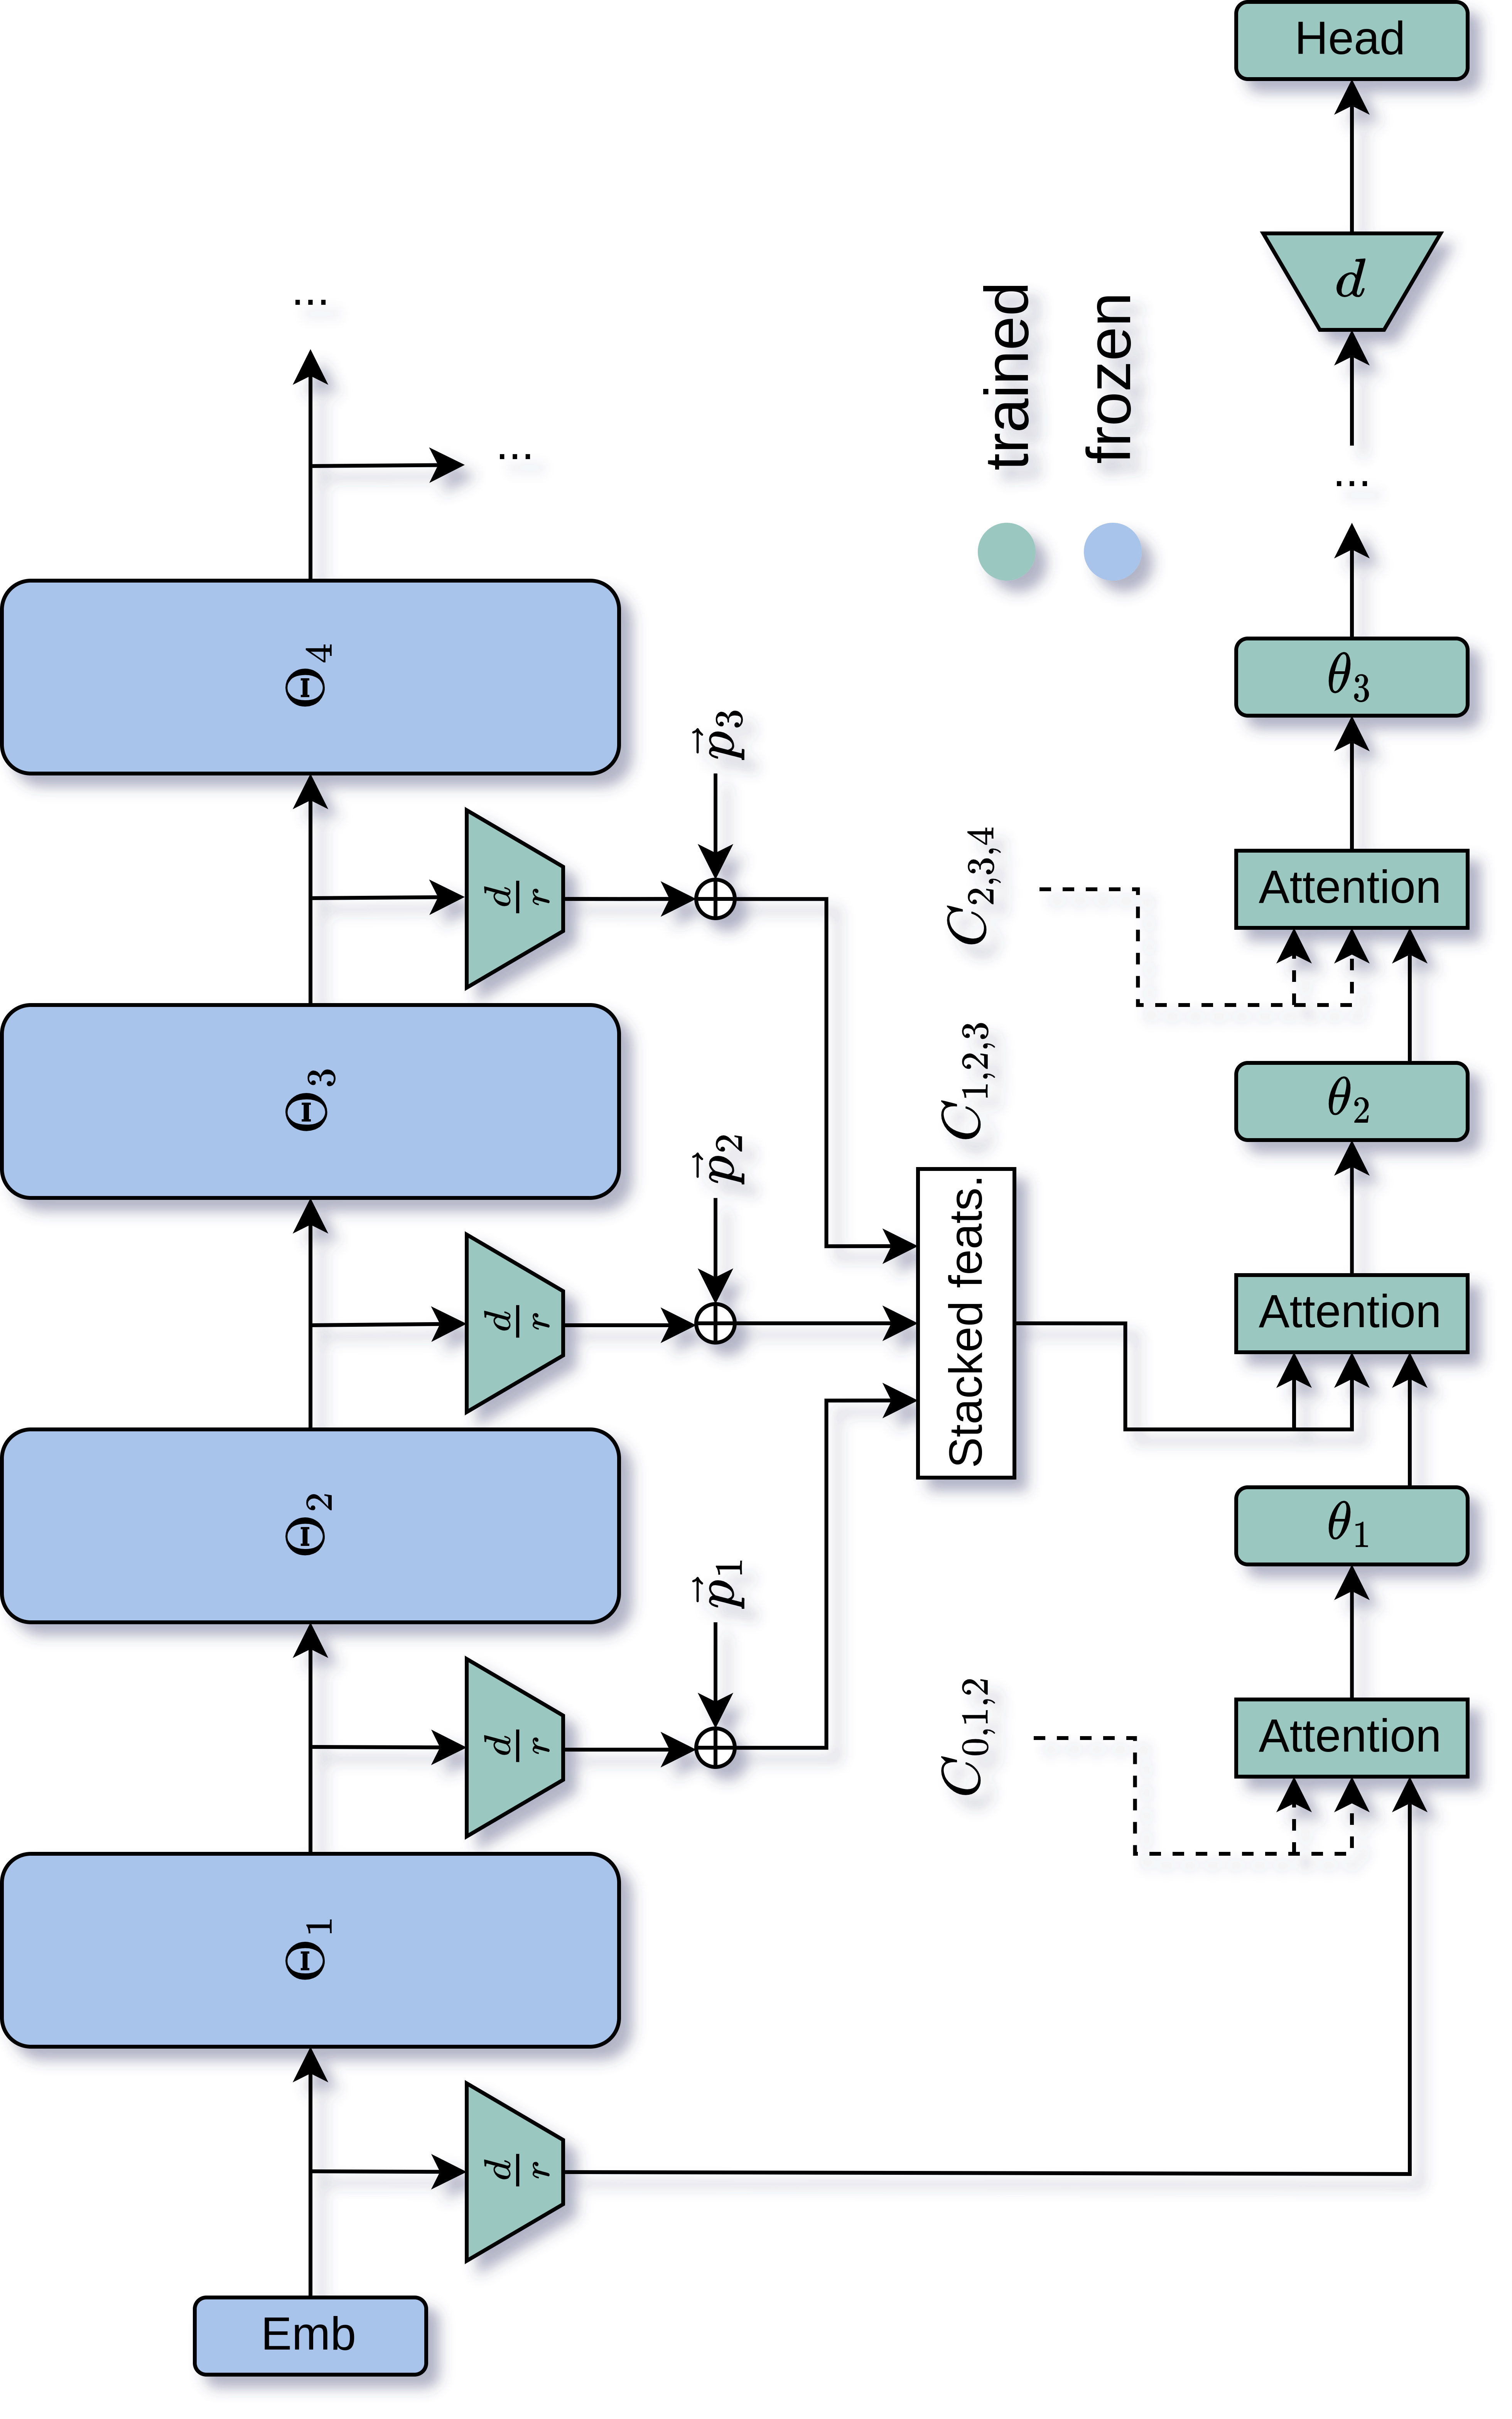
\includegraphics{assets/images/k-LST_rot.png}
    \end{adjustbox}
    \caption{k-LST diagram (k = 3)}
\end{figure}

\textbf{Advantages:}

\begin{itemize}[]
    \item No backpropagation through the base model
    \item Completely \textbf{unmodified base model} forward pass
    \item Comparable results to other PEFT methods at a \textbf{lower memory footprint}
    \item Tunable memory-performance tradeoff with $r$ and $k$
\end{itemize}

